\documentclass[12pt, letterpaper]{article}
\usepackage[english]{babel}

% include pdf
\usepackage[final]{pdfpages}

% quotes
\usepackage{csquotes}

% Acronyms
\usepackage[nopostdot,style=super,nonumberlist,toc,nogroupskip,acronym]{glossaries}

% For typesetting
\usepackage{lipsum}  

% Double spacing
\usepackage{setspace}

% Set paragraph spacing
\setlength{\parindent}{0pt}
\setlength{\parskip}{1em}
\def\ni{\noindent}

%% These two lines are needed to get the correct paper size
%% in TeX Live 2016
\let\pdfpageheight\paperheight
\let\pdfpagewidth\paperwidth

\makenoidxglossaries

\newacronym{auc}{AUC}{area under the receiver operating characteristic curve}
\newacronym{mam}{M\&M}{morbidity and mortality}
\newacronym{ml}{ML}{machine learning}
\newacronym{ofi}{OFI}{opportunity for improvement}
\newacronym{qi}{QI}{quality improvement}
\newacronym{gan}{GAN}{generative adversarial network}

\newglossaryentry{trauma}
{
    name=Trauma,
    text=trauma,
    description={Damage inflicted on the body as the direct or indirect result of an external force, with or without disruption of structural continuity.}
}

\newglossaryentry{gofi}
{
    name={OFI},
    text={OFI},
    description={Also known as opportunity for improvement}
}



% Acronym style
\newglossarystyle{csuper}{%
    \setglossarystyle{super}%
    \renewcommand{\glossentry}[2]{%
        \glsentryitem{##1}\glstarget{##1}{\glossentryname{##1}} &
        \Glossentrydesc{##1}\glspostdescription\space ##2\tabularnewline
    }
    \setlength{\glsdescwidth}{0.75\linewidth}
}

% Glossary style
\newglossarystyle{gsuper}{%
    \setglossarystyle{super}%
    \renewcommand{\glossentry}[2]{%
        \glsentryitem{##1}\glstarget{##1}{\glossentryname{##1}} &
        \Glossentrydesc{##1}\glspostdescription\space ##2\\[1em]
    }
    \setlength{\glsdescwidth}{0.65\linewidth}
}

% References
\usepackage[style=numeric,
    backend=biber,
    sorting=none,
    url=false,
    isbn=false,
    terseinits=true,
    giveninits=true,
    minnames=6,
    maxnames=6]{biblatex}

% Remove unwanted punctuations
\renewcommand*{\revsdnamepunct}{}
\renewcommand*{\finentrypunct}{}
\renewcommand*{\bibpagespunct}{}

% Dot instead av brackets in references
\DeclareFieldFormat{labelnumberwidth}{\mkbibbold{#1\adddot}}

% Lastname followed by initials format
\DeclareNameAlias{sortname}{family-given}
\DeclareNameAlias{default}{family-given}
\renewcommand*{\revsdnamepunct}{}

\DeclareSourcemap{%
    \maps[datatype=bibtex]{
        % Journal abbreviations
        \map[overwrite]{
            \step[fieldsource=shortjournal]
            \step[fieldset=journaltitle,origfieldval]
        }
    }
}

% remove in
\renewbibmacro{in:}{}
% remove pp
\DeclareFieldFormat*{pages}{#1}
% reformat doi
\DeclareFieldFormat*{doi}{\url{https://doi.org/#1}}
%remove quotation marks around title
\DeclareFieldFormat*{title}{#1}


\DeclareFieldFormat{journaltitle}{\mkbibemph{#1}\isdot}

% Provide three letter month names
\newcommand*{\shortmonth}[1]{
    \ifthenelse{\NOT\equal{#1}{}}{
        \ifcase#1\relax
        \or Jan
        \or Feb
        \or Mar
        \or Apr
        \or May
        \or Jun
        \or Jul
        \or Aug
        \or Sep
        \or Oct
        \or Nov
        \or Dec
        \fi
    }
}

\DeclareFieldFormat*{number}{\mkbibparens{#1}}

\DeclareFieldFormat*{date}{\thefield{year}}

% Code adapted from biblatex-nejm package

\renewbibmacro*{volume+number+eid}{
    \printfield{volume}%
    \setunit{}%
    \printfield{number}%
    \addcolon%
    \printfield{eid}%
}

\renewbibmacro*{issue+date}{
    \usebibmacro{date}
}

\renewbibmacro*{journal+issuetitle}{
    \usebibmacro{journal}%
    \iffieldundef{series}%
    \adddot%
    {}
    {\newunit%
        \printfield{series}}%
    \setunit{\addspace}%
    \usebibmacro{issue+date}%
    \setunit{\addsemicolon}%
    \usebibmacro{volume+number+eid}%
    \usebibmacro{issue}%
    \newunit}

% compress page numbers. E.g. XYZ-XAB -> XYZ-AB
\DeclareFieldFormat{postnote}{\mkcomprange[{\mkpageprefix[pagination]}]{#1}}
\DeclareFieldFormat{pages}{\mkcomprange{#1}}

% Compress ranges where lower limit > 100
\setcounter{mincomprange}{100}

% Don't compress beyond the fourth digit
\setcounter{maxcomprange}{1000}

% Display compressed upper limit with at least two digits,
% unless leading digit is zero
\setcounter{mincompwidth}{10} %imports biblatex 
\addbibresource{main.bib}


\begin{document}
\begin{titlepage}
    
\includepdf[pages=-,pagecommand={},fitpaper=true,]{title_page.pdf}
\end{titlepage}

\pagenumbering{Roman}

\textbf{Titel}

\lipsum[1]

\vfill

\textbf{Title}

\lipsum[1]

\vfill

\textit{Keywords}: Machine learning; Trauma; Medical audit; Trauma care quality improvement; Data synthesis; Prediction

\newpage

\glsaddall
\printnoidxglossary[type=acronym,style=csuper]
\printnoidxglossary[style=gsuper]

\newpage
\pagenumbering{arabic}

\doublespacing

\section{Introduction}
\Gls{trauma} is a major contributor to death and illness for individuals between the ages of 10 and 49 worldwide, and the leading cause of death amongst young people in Sweden \cite{roth_global_2018, vos_global_2020, sos_death_2021}. The \gls{trauma} population has a low average age and two-thirds of the group have no history of co-morbidity \cite{brattstrom_socio-economic_2015}. Thus it is essential to ensure a constant high-quality \gls{trauma} care to lower mortality and morbidity for this population with long a age expectancy.

A method of improving trauma patient care is to implement \acrfull{qi} programmes, as suggested by the World Health Organization (WHO) \cite{world_health_organization_guidelines_2009}. \Acrfull{mam} conferences are a cornerstone in such programmes and aim to identify \acrfull{ofi} in patient care \cite{santana_development_2014}. \acrshort{mam} conferences are conducted by representatives from all disciplines and professions involved in trauma care. During these conferences the treatment provided for an individual patient is discussed and compared against the optimal treatment that should have been provided. Regularly performing such reviews are associated with reducing complication frequencies, hospitalisation time, and preventable deaths; thus providing high-quality trauma care \cite{stelfox_evidence_2011, mcdermott_trauma_1994}. Due to the nature of \acrshort{mam} conferences however, they are extremely resource intensive \cite{}.

An \acrshort{ofi} is a concrete deficiencies in patient care and are often occur in initial care, such as, airway management, fluid resuscitation, haemorrhage control, and chest injury management \cite{world_health_organization_guidelines_2009,roy_learning_2017,oreilly_opportunities_2013,sanddal_analysis_2011}.

A more advanced \acrshort{qi} technique suggested by WHO is the application of audit filters that use electronic health record systems to monitor predefined variables to flag cases with \acrfull{ofi} \cite{world_health_organization_guidelines_2009}. Filtering cases using an audit filter before reviewing by an \acrshort{mam} conference provides a possibility to reduce false positive cases and thus reducing the costs of the \acrshort{qi} programme as a whole.

However, the performance of such systems varies and have been associated with high frequencies of false positives. Depending on context the frequency of false positives can range from 24\% to 80\% \cite{attergrim_predicting_2023,sanddal_analysis_2011,roy_learning_2017,ghorbani_analysis_2018}.

A new method suggested by Attegrim and Szolnoky et al. suggests to replace audit filter systems with supervised \acrfull{ml} models \cite{attergrim_predicting_2023}. These newer models achieve a significantly better performance than the currently used audit filter system at Karolinska University Hospital in Stockholm, Sweden. At the same sensitivity, the false positive rate is reduced from 68\% to 53\% using the same data.

Despite this performance boost, the models' still suffer from that 50\% of patient cases are incorrectly flagged as \acrshort{ofi} positive. \acrshort{ml} methods in general require large amounts of data to be able to perform \cite{}. Many methods exist to increase the performance of \acrshort{ml} models, and perhaps the most fundamental and well known is simply increasing the sheer amount of data. So far, the only possible method in doing so was by manually collecting more data and annotating it. This is a slow process, and in some cases not possible due to the fundamental lack of data.

\begin{figure}[t]
    \centering
    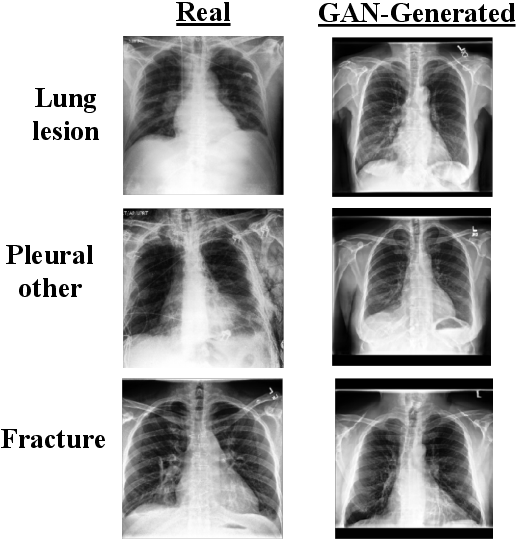
\includegraphics[width=0.6\textwidth]{figures/gan-xray.png}
    \caption{Example of using a \acrfull{gan} to generate chest radiograph images. Image taken from \cite{}.}
    \label{fig:gan-xray}
\end{figure}

Recently however, using \acrfullpl{gan} to generate synthetic data has become a hot topic in image analysis \cite{}. A \acrshort{gan} is a type of artificial neural network. \acrshortpl{gan} internally use two neural networks, one network to generate data (the generator) and another that tells how realistic the data is compared to the ground truth data (the descriminator). During the training of \acrshortpl{gan}, the two internal models constantly compete; the generator model generating data that the descriminator can't tell apart from the ground truth data. \cite{}. \acrshortpl{gan} can be seen as a sort of evolutionary arms race between the two internal models, similar to the evolutionary process known as mimicry. In short,by training a \acrshort{gan} on true manually annotated data one can there after produce more data.

The quality of the generated data often varies and depends on several factors, such as, the quality and amount of ground truth data \cite{}. The major benefit of having a method for generating quality synthetic data is the possibility of expanding small datasets and training \acrshort{ml} models where it was not previously possible or did not achieve adequate results due to data amount.

In addition to generating more trainable data, most \acrshortpl{gan} are able to anonymise data \cite{}. Thus providing an interface for being able to generate synthetic datasets of sensitive personal information that are completely anonymous. These synthetic datasets can, in theory, be distributed and increase the availability of medical datasets for researchers.

\subsection{Aim}
Hitherto, using \acrshortpl{gan} is rare and relatively unexplored for structured tabular data. Few articles exist investigating the feasibility of generating synthetic tabular data in a medical context.

Therefore, the aim of this article is to evaluate the effectiveness of using \acrshortpl{gan} for generating synthetic tabular data in a trauma setting, and to investigate the potential of this approach for improving \acrshort{ofi} prediction models.

\section{Materials and Methods}
We conducted a registry-based study using all trauma patients included in Karolinska University Hospital trauma registry and trauma care quality database between 2014 and 2021 to compare the performance of supervised \acrshort{ml} models trained with and without synthetic data.

\subsection{Study Population and Setting}

\subsection{Predictor Variables}

\subsection{Outcome variable}

\subsection{Model Development}

\subsection{Statistics Analysis}

\subsection{Ethical Considerations}
The study was approved by Stockholm Research Ethics Review Board, approval number 2021-02541 and 2021-03531.

\section{Results}

\section{Discussion}

\section{Conclusions}

\section*{Contributions}

\section*{Acknowledgement}

\singlespacing

\printbibliography

\end{document}